\documentclass[12pt, a4paper]{article}

\usepackage{lipsum}% http://ctan.org/pkg/lipsum
\setlength{\parindent}{1.25cm}

\usepackage{hyperref}
\hypersetup{
    colorlinks=true, % make the links colored
    linkcolor=black, % color TOC links in blue
    urlcolor=red, % color URLs in red
    linktoc=all % 'all' will create links for everything in the TOC
}
\usepackage{mathtext}
\usepackage[T2A]{fontenc}  % поддержка кириллицы в ЛаТеХ
\usepackage[utf8]{inputenc} % кодировка
\usepackage[english, russian]{babel} % определение языков в документе
% \usepackage{pscyr} % красивые кириллические шриф ты
% \usepackage{mathspec}
% \usepackage{upgreek} % добавляет прямые греческие символы
\usepackage[eulergreek, italic]{mathastext}
% \usepackage{lscape} % для включения альбомных страниц (широкие таблицы, графики и т.д.)

% \usepackage{nath}

\usepackage{amsmath} % многострочные формулы
% \usepackage{breqn}  % автоматические многострочные формулы
\usepackage{amstext} % определяет \textit{} для включения в формулы текста
\usepackage{amssymb} % набор символов
% \usepackage{makecell} % работа с ячейками в таблицах
% \usepackage[math-style=upright]{unicode-math}
\usepackage{indentfirst}  % делает отступ в начале параграфа

% \usepackage{lmodern}
% \usepackage{listings} % для листингов программ
\usepackage{pdflscape} % альбомные страницы

\usepackage{longtable} % для многостраничных таблиц
\usepackage{multirow}  % для объединения ячеек таблиц
\usepackage{multicol}  % для объединения ячеек таблиц

\usepackage{mathtools}
% \usepackage{makeidx}
% \usepackage{amssymb}
% \usepackage{amsfonts}
\usepackage{cite}
% \usepackage{hyperref}

\usepackage{enumerate} % нумерация списков
\usepackage{enumitem}

% \usepackage{txfonts}
% \usepackage{kpfonts}

% \usepackage{float}
% \usepackage{mathdots}
% \usepackage{pdflscape}
\usepackage{array}

\pagestyle{empty}

% \usepackage{ltxtable}
% \usepackage{lipsum}

\usepackage{geometry} % размеры листа
\geometry{left = 3cm} % размеры листа
\geometry{right = 2cm} % размеры листа
\geometry{top = 2cm} % размеры листа
\geometry{bottom = 2cm} % размеры листа

\usepackage[figurename=Рисунок]{caption}
\usepackage{subcaption}

\DeclareCaptionLabelFormat{continued}{Продолжение таблицы~#2}
\DeclareCaptionLabelFormat{gostfigure}{Рисунок #2}
\DeclareCaptionLabelFormat{gosttable}{Таблица #2}
\DeclareCaptionLabelSeparator{gost}{~---~}

\captionsetup[figure]{justification = centering}
\captionsetup{labelsep=gost}
\captionsetup*[figure]{labelformat=gostfigure}

\usepackage{graphicx}
% \setlength\extrarowheight{6pt}

\renewcommand{\rmdefault}{ftm} % переключение на общий шрифт документа Times New Roman (пакет pscyr)
%\renewcommand\theadfont{\normalsize}

\linespread{1.3}

\frenchspacing

% \usepackage{tikz}
% \usetikzlibrary{shapes.geometric, arrows}
% \usetikzlibrary{automata,positioning}


\usepackage{titlesec}

% Настройка формата разделов и подразделов
\titleformat{\section}{\normalfont\normalsize\bfseries}{\thesection}{1em}{}
\titleformat{\subsection}{\normalfont\normalsize\bfseries}{\thesubsection}{1em}{}
\titleformat{\subsubsection}{\normalfont\normalsize\bfseries}{\thesubsubsection}{1em}{}

% Настройка расстояния до разделов и подразделов и после
\titlespacing*{\section}{\parindent}{0pt}{18pt}
\titlespacing*{\subsection}{\parindent}{18pt}{18pt}
\titlespacing*{\subsubsection}{\parindent}{18pt}{18pt}

% Каждый раздел с новой страницы
\newcommand{\sectionbreak}{\clearpage}

% \addto\captionsenglish{
% \renewcommand\contentsname{СОДЕРЖАНИЕ}
% }
\addto\captionsrussian{
    \renewcommand\contentsname{\hfill СОДЕРЖАНИЕ\hfill}
}

%\usepackage{accsupp}

\makeatletter
\renewcommand*\l@section{\@dottedtocline{1}{1.5em}{2.3em}}
\renewcommand*\l@subsection{\@dottedtocline{1}{1.5em}{2.3em}}
\renewcommand*\l@subsubsection{\@dottedtocline{1}{1.5em}{2.3em}}
% \newcommand\cdot {\copyable}{%
%   \begingroup
%   \@sanitize
%   \catcode`\%=14 % allow % as comment char, also needed for \%
%   \@copyable
% }
% \newcommand\cdot {\@copyable}[1]{%
%   \endgroup
%   \BeginAccSupp{%
%     ActualText=\detokenize{#1},%
%     method=escape,
%   }%
%   \scantokens{#1}%
%   \EndAccSupp{}%
% }
\makeatother



\begin{document}

\begin{titlepage}

\begin{center}
Министерство образования и науки Российской Федерации\\
Федеральное государственное автономного образовательное учреждение высшего образования\\
\hrulefill\\
\vspace{0.5cm}
САНКТ-ПЕТЕРБУРГСКИЙ ПОЛИТЕХНИЧЕСКИЙ УНИВЕРСИТЕТ\\ ПЕТРА ВЕЛИКОГО\\
\vspace{0.5cm}
Институт Энергетики\\
Высшая школа энергетического машиностроения\\

\end{center}

\vspace{5cm}
\begin{center}
\begin{large}
Лабораторная работа №2\\
"Определение частот собственных колебаний вращающегося диска"
\end{large}
\end{center}

\vspace{5cm}
\hspace{5cm} Студент гр. 3231303/81001 \hrulefill Степанов С.С.


\vspace{0.5cm}
\hspace{5cm} Преподаватель \hrulefill Курнухин А.А. \\


\vfill
\begin{center}
Санкт-Петербург\\
2021
\end{center}


\end{titlepage}

\tableofcontents
\newpage

\section{Теория}
Частота собственных колебаний ротора зависит от частоты вращения ротора. Это явление объясняется действием гироскопического момента, возникающего при вращении ротора с дисками. При прямой прецессии (явление смещения геометрического центра ротора в плоскости, которая перпендикулярна оси ротора, в направлении вращения ротора; Рисунок 1) гироскопический момент стремится вернуть диск в исходное положение, т.е. он увеличивает возвращающий момент, что эквивалентно увеличению жёсткости. Таким образом, гироскопический момент при прямой прецессии увеличивает жёсткость вала и, как следствие, все его собственные частоты колебания и критические частоты.\\

\begin{figure}[h]
\center
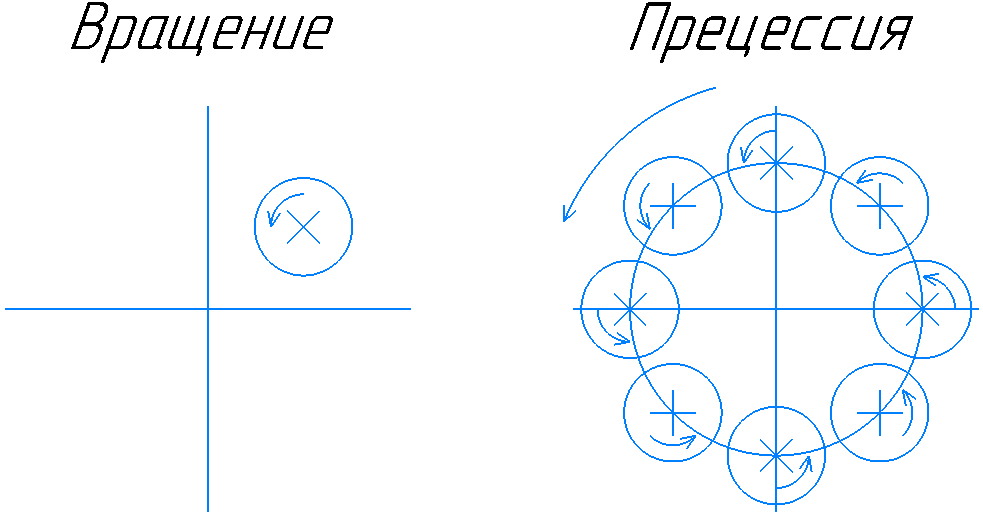
\includegraphics[width=120mm]{prec.png}
\caption{Явление прямой прецессии} \label{fig:1}
\end{figure}

В ходе данной лабораторной работы был произведен расчет собственной частоты поперечных колебаний ротора с диском, а так же графически построена зависимость собственной частоты поперечных колебаний ротора от частоты его вращения . 

\section{Исходные данные}

Длина ротора, [м]

\[l = 1,24.\]

Диаметр ротора, [мм]

\[d = 46.\]

Диаметр диска, [мм]

\[D = 220.\]

Толщина диска, [мм]

\[h = 29.\]

Плотность стали, [кг/м\textsuperscript{3}]

\[\rho = 8000.\]

Модуль упругости, [МПа]
\[Е = 20000.\]


\section{Определение собственных частот поперечных колебаний системы,
  расположенной на вращающемся диске}

Масса диска, [кг]

\[m = \rho\cdot V = \rho\cdot\frac{\pi\cdot D^{2}}{4}\cdot h = 8000\cdot\frac{3,14\cdot({220\cdot10^{- 3})}^{2}}{4}\cdot29\cdot10^{- 3} = 8,81.\ \]

Полярный момент инерции, [ м\textsuperscript{4}]

\[Y_{\text{xx}} = \frac{\pi\cdot d^{4}}{64} = \frac{3,14\cdot({46\cdot10^{- 3})}^{4}}{64} = 2,198\cdot10^{- 7}.\ \]

Податливость, [м/Н]

\[\delta_{11} = \frac{P\cdot{(2\cdot l)}^{3}}{48\cdot E\cdot Y_{\text{xx}}} = \frac{1\cdot{(2\cdot1,24)}^{3}}{48\cdot2\cdot10^{11}\cdot2,198\cdot10^{- 7}} = 7,23\ \cdot10^{- 6}.\ \]

Собственная частота поперечных колебаний, [Гц]

\[p = \sqrt{\frac{1}{\delta_{11}\cdot m}} = \sqrt{\frac{1}{7,23\ \cdot10^{- 6}\cdot8,81}} = 125,24\ \frac{рад}{с} = 19,93.\ \]

\(p_{\omega} = \sqrt{p_{0}^{2} + w_{p}^{2}\cdot\frac{R}{l}\ }\) =
\(\sqrt{{125,24}^{2} + 314^{2}\cdot2,3}\) = \(492,39\ рад/с = 78,37.\ \)
\newpage

\section{Оценка влияния вращения на частоту собственных колебаний}

Составим таблицу:

\begin{center}
\begin{tabular}{ccc}
& \(\omega\) & \(p_{\omega}\)\\
0 & 0 & 125,24\\
0,25\(w_{p}\) & 78,5 & 172,79\\
0,5\(w_{p}\) & 157 & 269,03\\
0,75\(w_{p}\) & 235,5 & 378,48\\
\(w_{p}\) & 314 & 492,40\\
\end{tabular}
\end{center}

Построим график:
\begin{figure}[h]
\center
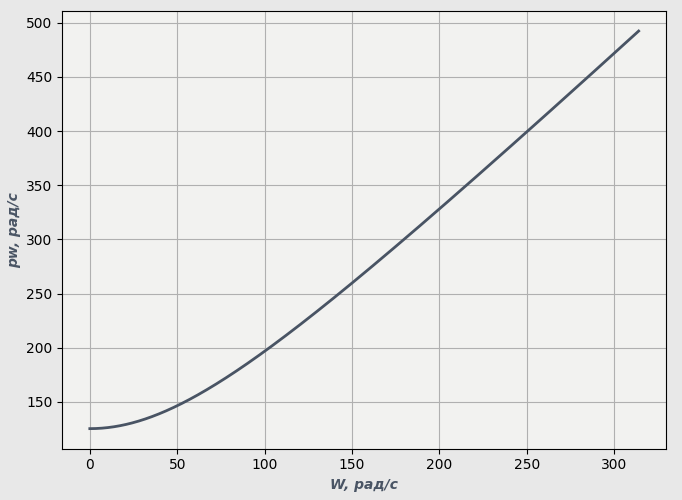
\includegraphics[width=120mm]{graph.png}
\caption{Зависимость частоты собственных колебаний диска от частоты вращения ротора} \label{fig:2}
\end{figure}

По графику, изображенному на Рисунке 2, можно определить, что зависимость частоты собственных колебаний от угловой скорости вращения остается нелинейной только в самом начале кривой (на участке от 0 рад/с до 100 рад/с).

\section{Список использованной литературы}

1. Костюк А.Г.Динамика и прочность турбомашин: Учебник для вузов.  Москва.: Издательский дом МЭИ, 2007. 477 с.

\end{document}
